\documentclass{report}
\usepackage[francais ]{babel}
\usepackage[utf8]{inputenc}
\usepackage[T1]{fontenc}
\usepackage{graphicx}
\usepackage{float}
\usepackage{hyperref}
\usepackage{array}
\title{\Huge Guide d'utilisateur \\ \huge Mini Games }

\author{M. \textsc{Friedli}, A. \textsc{Gillioz}, J. \textsc{Guerne}\\
He-Arc Ingénierie\\
2000 Neuchatel}
\date{\today{}}
\begin{document}
\maketitle

\chapter{Connexion}
Pour commencer à jouer il faut commencer par se connecter à un serveur.
Au lancement du programme vous devrez donc entrer l'adresse d'un serveur et aussi chsoir un pseudo. Une fois les champs remplis vous pouvez cliquer sur le bouton connecter pour tenter de vous connecter.

\begin{figure}[H]
	\centering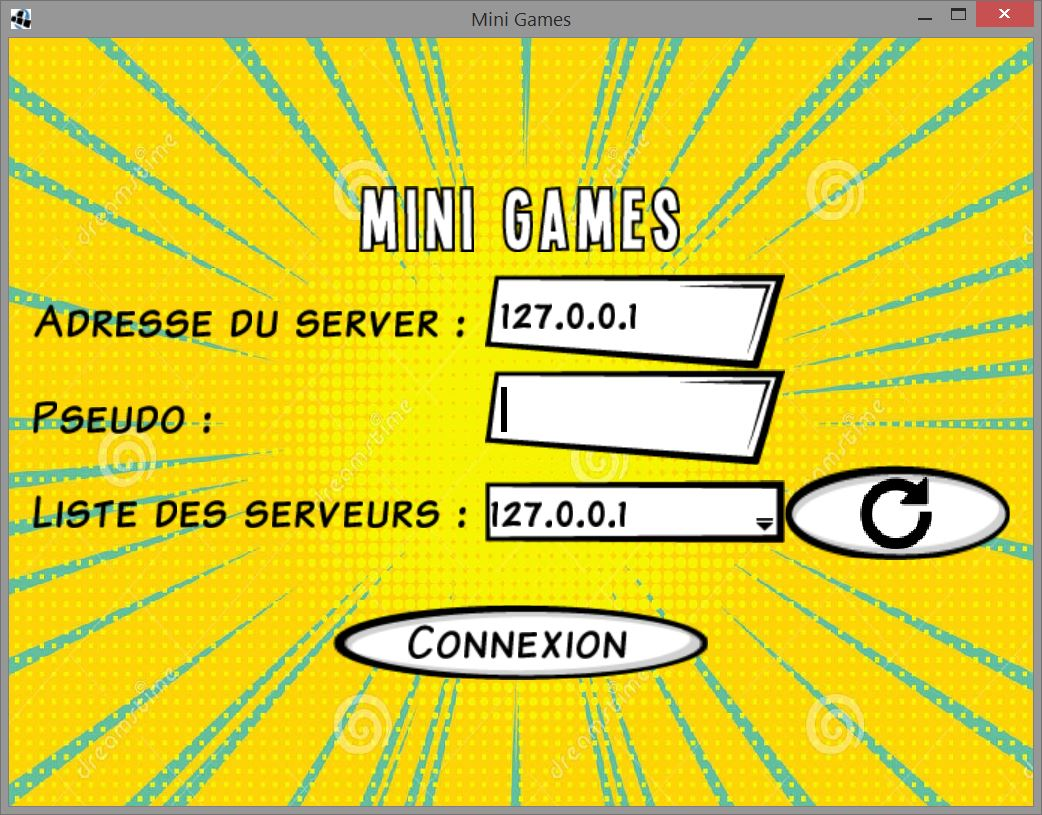
\includegraphics[width=9cm]{loginScreen}
	\caption{Écran de connexion}
\end{figure}

Pour faciliter la connexion au sevreur un système de recherche des serveurs est disponible. Le recherche se lance
automatiquement au démarrage du programme et peut être relancé à nouveau plus tards en appuyant sur le bouton de rafraichissament.


\chapter{Menu de sélection des minis jeux}
Une fois correctement connecté au serveur vous avez le choix de lancer une partie de morpion ou de bataille navale.
\begin{figure}[H]
	\centering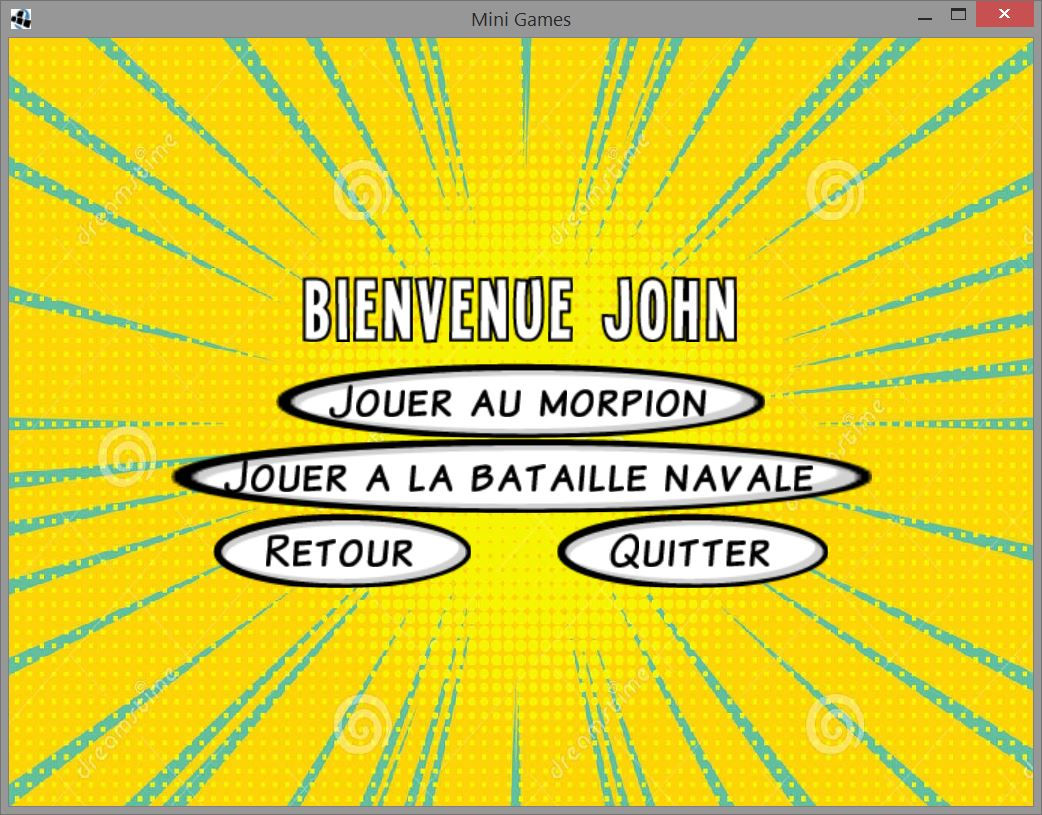
\includegraphics[width=9cm]{MenuJeux}
	\caption{Écran de connexion}
\end{figure}

Quand vous commencez une partie d'un jeu vous êtes dabord mis en attente puis
une fois un adversaire trouvé la partie commencera.

\begin{figure}[H]
	\centering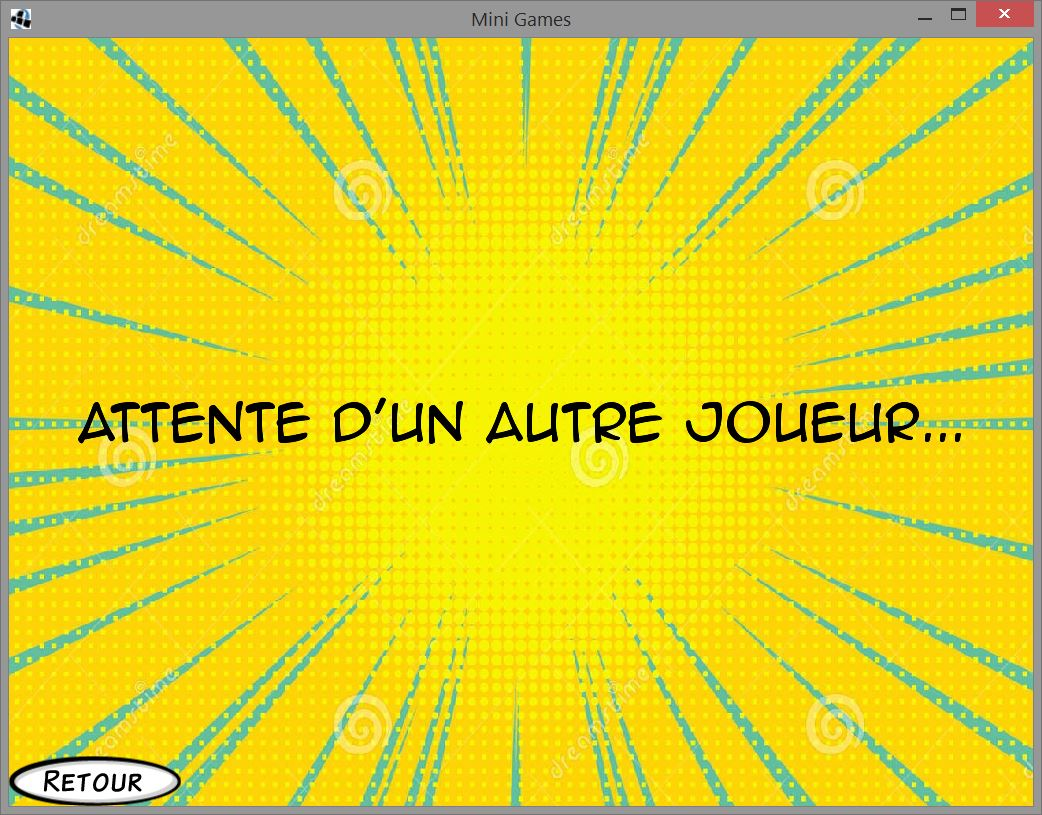
\includegraphics[width=9cm]{morpionwaiting}
	\caption{Écran d'attente}
\end{figure}



\chapter{Morpion}



\chapter{Bataille navale}

\end{document}
